\documentclass{vgtc}                          % final (conference style)

\ifpdf%                                % if we use pdflatex
  \pdfoutput=1\relax                   % create PDFs from pdfLaTeX
  \pdfcompresslevel=9                  % PDF Compression
  \pdfoptionpdfminorversion=7          % create PDF 1.7
  \ExecuteOptions{pdftex}
  \usepackage{graphicx}                % allow us to embed graphics files
  \DeclareGraphicsExtensions{.pdf,.png,.jpg,.jpeg} % for pdflatex we expect .pdf, .png, or .jpg files
\else%                                 % else we use pure latex
  \ExecuteOptions{dvips}
  \usepackage{graphicx}                % allow us to embed graphics files
  \DeclareGraphicsExtensions{.eps}     % for pure latex we expect eps files
\fi%

%% it is recomended to use ``\autoref{sec:bla}'' instead of ``Fig.~\ref{sec:bla}''
%\graphicspath{{figures/}{pictures/}{images/}{./}} % where to search for the images
 \usepackage[utf8]{inputenc}
 
\usepackage{microtype}                 % use micro-typography (slightly more compact, better to read)
\PassOptionsToPackage{warn}{textcomp}  % to address font issues with \textrightarrow
\usepackage{textcomp}                  % use better special symbols
\usepackage{mathptmx}                  % use matching math font
\usepackage{times}                     % we use Times as the main font
\renewcommand*\ttdefault{txtt}         % a nicer typewriter font
\usepackage{cite}                      % needed to automatically sort the references
\usepackage{tabu}                      % only used for the table example
\usepackage{booktabs}                  % only used for the table example
\usepackage{listings}				   % Para insertar el codigo de programcion
\usepackage{graphicx}

\onlineid{0}

\vgtccategory{Research}

\vgtcinsertpkg


\title{Learning PAC}

\author{Andres J. Montenegro Bello\thanks{e-mail: montenegroandresj@gmail.com}\\      \scriptsize GitHub : AndresJuniorMontenegro%
\and Raul Huaman Pajares \thanks{e-mail: rahuamanpa@gmail.com }\\ %
     \scriptsize GitHub : rhuamanpa\\
\and Repositorio \\
     \scriptsize https://github.com/rhuamanpa/Pac-Learning
}

%% Abstract section.
\abstract{ We will analize PAC learning, the type of uses that we can apply with PAC learning with machine learning and show some samples used by big companies like Facebook and Youtube to make incomes at the same time we will make a project using PAC learning using python that will recognize some facial gestures.%
} % end of abstract

%%%%%%%%%%%%%%%%%%%%%%%%%%%%%%%%%%%%%%%%%%%%%%%%%%%%%%%%%%%%%%%%
%%%%%%%%%%%%%%%%%%%%%% START OF THE PAPER %%%%%%%%%%%%%%%%%%%%%%
%%%%%%%%%%%%%%%%%%%%%%%%%%%%%%%%%%%%%%%%%%%%%%%%%%%%%%%%%%%%%%%%%

\begin{document}

\firstsection{Introduction}

\maketitle

%% \section{Introduction} %for journal use above \firstsection{..} instead
La probabilidad aproximada correcta (PAC), propuesta por L.Valiant,
es un marco de referencia estatico para aprender usar datos de entrenamiento.
\\
\\
En su forma mas simple y para un modelo tipico de tarea, la teoria
del aprendizaje PAC intentan relacionar, precision y confianza 
estadistica del modelo al numero de ejemplos de entrenamientos 
usados.
\\
\\
Uno de los conceptos más importantes en este sentido es medir la
complejidad de una clase de hipótesis $H$. En cualquier modelo de
aprendizaje automático, el objetivo final es encontrar una clase de
hipótesis que logre una alta precisión en el conjunto de
entrenamiento y que tenga un bajo error de generalización en el conjunto
de prueba. Para esto, requerimos que la clase de hipótesis $H$ se
aproxime al concepto de clase $C$ que determina las etiquetas para la
distribución $D$. Como tanto $C$ como $D$ son desconocidos, tratamos
de modelar $H$ en base al conjunto de muestras conocido $S$ y sus etiquetas.

\textbf{Generalizacion del error: }
El error de generalización de una hipótesis $h$ es la expectativa del
error en una muestra $x$ elegida de la distribución $D$.

\textbf{Error empirico: }
Esta es la media del error de la hipótesis $h$ en la muestra $S$ del 
tamaño $m$.

Habiendo definido el error de generalización y el error empírico de
esta manera, podemos establecer el objetivo del aprendizaje de la
siguiente manera.
\newline
\newline
\textit{El objetivo del aprendizaje es tener el error empírico
aproximado al error de generalización con alta probabilidad.}
\newline
\newline
Este tipo de marco de aprendizaje se conoce como Aprendizaje PAC
(Probablemente Aproximadamente Correcto). Formalmente, una clase de
concepto $C$ es $PAC-aprendible$ si hay algún algoritmo $A$ para el 
cual el error de generalización en una muestra $S$ derivado de la 
distribución $D$ es muy bajo (menor que $\epsilon$) con alta 
probabilidad (mayor que $1- \delta$). En otras palabras, podemos decir que para una
clase apta para PAC, la precisión es alta con buena confianza.
\\
\\
Se adjuntara una imagen en la cual dara una descripcion general del aprendizaje PAC.
\\
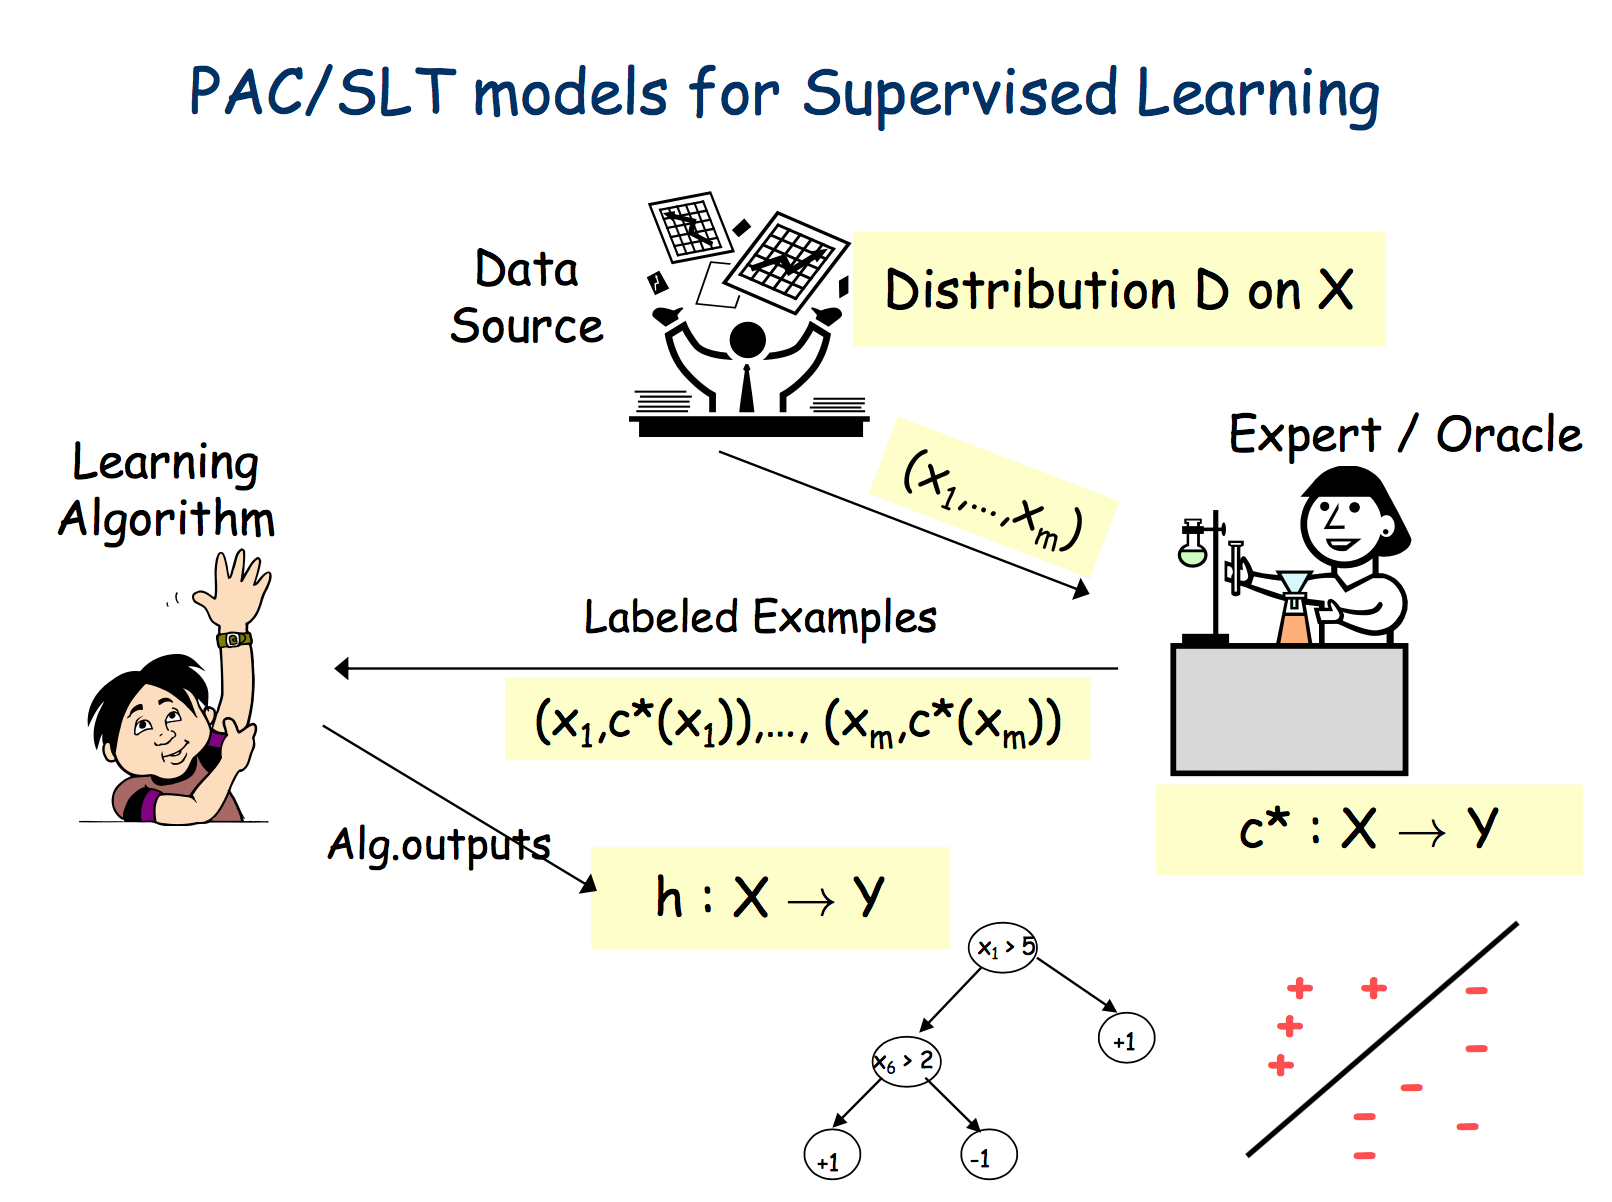
\includegraphics[scale=0.15]{pac.png} 
\section{Estado del arte}

El aprendizaje PAC( aprendizaje correcto probablemente aproximado) como su
nombre lo dice generara probables situaciones para dar un resultado
correcto aproximado, esta ciencia es una similitud o podemos decir una
rama del machine learning y el deep learning, sus usos son muy dinamicos y
eficaces, actualmente se utiliza como herramienta muy util veamos 3
ejemplos:
\newline
\newline
\textbf{Identificación de temas: }
Clasificación multi-etiqueta de medio de articulos impresos deducido
de una base de datos.
\newline
\newline
La data fue recolectada desde el Mayo del 2013 hasta Setiembre del 2013,
\newline
\newline
Los articulos fueron manualmente segmentados.
\newline
\newline
El texto de los articulos es representado usando \textit{"Una mochila de
palabras modelo "}.
\newline
\newline
Esta base de datos cuenta con $301 561$ atributos numericos, $213$ tipo de
etiqueta y $99 780$ articulos, los cuales $64 857$ fueron data de 
entrenamiento y $34 923$ fueron data de prueba, el objetivo es predecir 
las etiquetas relevantes del conjunto de data de prueba.
\newline
\newline
Se adjunta el link del conjunto de data:
\newline
\newline
\url{https://www.kaggle.com/c/wise-2014/data}
\newline
\newline

\textbf{Recomendación de peliculas: }
Sistema utilizado para predecir la afluencia que tendra una pelicula y su calificacion 
global, determinada por la calificacion previa a peliculas con similar caracteristica 
o etiqueta sacada de una base de datos ya sea de \textit{Netflix} o \textit{Movie Lens}
\newline
\newline
Se adjuntara los links de la base de datos de dichas plataformas de peliculas:

\textit{Netflix: \\}  \url{https://www.netflixprize.com/leaderboard.html}
\newline
\newline
\textit{Movie Lens:\\ } \url{https://grouplens.org/datasets/movielens/}
\newline
\newline

\textbf{Video resumen: }
Selecciona semanticamente las partes más importantes de un video
debido a una base de datos muy grande de metricas en la plataforma 
de $YOUTUBE$, esto es usado como grandes compañias como \textit{Facebook y Youtube}, para que puedan insertar la publicidad
en las partes mas relevantes del video subido y asi más probabilidad
de que puedan ver la publicidad.
\newline
\newline
Se adjunta la data de \textit{Youtube} y es : \newline \newline
\url{https://research.google.com/youtube8m/index.html}


\section{Diseño del experimento}

Se diseñara un experimento en la cual se capturara una imagen
y este reconocera ciertos gestos faciales.
\\
\\
Debido a un conjunto de patrones establecidos.
\\
\\
Se implementara con el lenguaje de programación \textit{Python.}


\section{Experimentos y Resultados}

\begin{itemize}

\item Para realizar el reconocimiento facial se usara el lenguaje de programación Python.

\item Se usara extensiones a ciertas librerias como:
	
	\begin{itemize}
	\item Libreria OpenCV
	\item Libreria Numpy
	\item Libreria PIL
	\item Libreria Pickle
	\end{itemize}

\subsection{Primera etapa}

\item Para empezar el experimento al instalar la libreria OpenCV, esta misma librearia nos proporciona de una data para aplicar el reconocimiento de los rostros que se llama \textbf{harrcascade\_frontalface\_alt2.xml}

\item El proceso del experimento requerrira de dos ficheros donde uno de ellos es para el entrenamiento y el otro usara el entrenamiento para aplicar el reconocimiento facial.

\end{itemize}

\begin{itemize}

\item Empezaremos el codigo primero con tener el control de la camara de video de la Laptop en este caso.

\begin{lstlisting}

import cv2

cap = cv2.VideoCapture(0)

while (True):

    #Capturar frame por frame
    ret,frame = cap.read()
   
    #Mostrando los frames resultantes
    cv2.imshow('frame',frame)

    if cv2.waitKey(20) & 0xFF==ord('q'):
        break

cap.release()
cv2.destroyAllWindows()
\end{lstlisting}

\item Una vez que se pudo tener la captura de video pasariamos a usar la data que nos proporciona la libreria OpenCV

\begin{lstlisting}

face_cascade = cv2.CascadeClassifier("cascade
/data/haarcascade_frontalface_alt2.xml")

\end{lstlisting}

\item Una vez utilizando la data que nos da la librearia OpenCV, seguimos a pasar los \textbf{frame} capturados a escala de color gris.

\begin{lstlisting}

gray = cv2.cvtColor(frame,cv2.COLOR_BGR2GRAY)

\end{lstlisting}

\item Luego se procede a reconocer la existencia de rostros


\begin{lstlisting}
faces = face_cascade.detectMultiScale(gray,
	scaleFactor=1.5, minNeighbors=5)
\end{lstlisting}

\item Despues dibujariamos un rectangulo en el rostro reconocido, y en la libreria OpenCV utiliza los colores de forma BGR (Blue, Green, Red) y no la forma tradicional RGB.

\begin{lstlisting}
for (x,y,w,h) in faces:
  color = (255,0,0)
  stroke = 2
  end_cord_x = x+w
  end_cord_y = y+h
  cv2.rectangle(frame,(x,y),
     (end_cord_x,end_cord_y),
     color,stroke)
\end{lstlisting}

\item Con todo estos pasos se puede reconocer rostros gracias a la libreria OpenCV y a la data que ofrece
para reconocer rostros.

\item El fichero de todo esto se encuentra con el nombre de \textbf{captura\_rostro.py}

\begin{figure}[h]
	\centering
	\includegraphics[scale=0.15]{prueba1.png}
	\caption{Prueba de reconocimiento de rostro}
\end{figure}

\end{itemize}

\subsection{Segunda etapa}

\begin{itemize}

\item Lo que sigue, es ahora crear una pequeña base de datos de imagenes, en este caso usaremos imagenes de personajes de una serie quienes son:

	\begin{itemize}
	\item Harvey Specter
	\item Donna
	\item Michael Ross
	\end{itemize}

\item De cada personaje usamos 6 imagenes que se encuentra en carpetas que son sus respectivos nombres.

\item Para empezar el entrenamiento tenemos que referenciar sus ubicaciones absolutas de todas las fotos que usaremos para hacer la prueba.

\begin{lstlisting}
#Obtener las direcciones absoluta del 
#directorio del fichero
BASE_DIR = os.path.dirname(
   os.path.abspath(__file__))

#Dentro de ese fichero hay una carpeta 
#images y ahi estan las imagenes de los 
#personajes

image_dir = os.path.join(BASE_DIR,"images")
\end{lstlisting}


\item Despues de ello extraemos todos las direcciones abslutas de todas las imagenes de los personajes.

\begin{lstlisting}
for root,dirs,files in os.walk(image_dir):
  for file in files:
     if file.endswith("png") or 
           file.endswith("jpg"):
        path = os.path.join(root,file)
        label = os.path.basename(root).
                replace(" ","-").lower()
\end{lstlisting}

\item Convertimos a escala grises todas las imagenes de los personajes con la libreria PIL y lo guardamos en un array de imagenes.

\begin{lstlisting}
#Escala grises
pil_image = Image.open(path).convert("L") 
image_array = np.array(pil_image,"uint8")
\end{lstlisting}

\item Lo mismo que en la primera etapa usaremos la data de OpenCV nos ofrece para reconocer los rostros de las imaegenes de los personajes seleccionados.

\begin{lstlisting}
face_cascade = cv2.CascadeClassifier("
  cascade/data/haarcascade_frontalface
  _alt2.xml")
\end{lstlisting}

\item Despues con todas las imagenes dentro de image\_array se seguira con los rostros detectados en dichas imagenes.

\begin{lstlisting}
faces = face_cascade.detectMultiScale(
   image_array,scaleFactor=1.5, 
   minNeighbors=5)
            
\end{lstlisting}

\item Despues se guarda los rostros reconocidos en un vector \textbf{x\_train} y su etiqueta en \textbf{y\_labels}.

\begin{lstlisting}
for (x,y,w,h) in faces:
   roi = image_array[y:y+h, x:x+w]
   x_train.append(roi)
   y_labels.append(id_)
            
\end{lstlisting}

\item Por ultimo exportamos dos archivos.

\item El primer archivo es para las etiquetas de cada carpeta de fotos, que en otras palabras seria el nombre del personaje con su respectiva foto y este archivo se llama \textbf{labels.pickle}

\item El segundo archivo es aquel que sirvira para el entrenamiento y asi poder reconocer los rostros de los personajes seleccionados y este archivo se llama \textbf{trainner.yml}

\item El archivo de entrenamiento de rostros se llama \textbf{entrenamiento\_rostros.py}

\begin{figure}[h]
	\centering
	\includegraphics[scale=0.3]{prueba2.png}
	\caption{Ficheros de entrenamiento}
\end{figure}

\end{itemize}

\subsection{Tercera etapa}

\begin{itemize}

\item Una vez teniendo los archivos de entrenamiento ahora haremos los cambios respectivos para el fichero de la primera etapa.

\item Se crea un variable que extraiga la informacion del archivo "trainner.yml" ya que es el archivo para que reconozca a los personajes escogidos previamente.

\begin{lstlisting}
recognizer = cv2.face.LBPHFace
   Recognizer_create()

recognizer.read("trainner.yml")            
\end{lstlisting}

\item Luego se captura las etiquetas o nombres de los personajes escogidos del archivo "labels.pickle" para que me arroje el nombre del rostro de dicho personaje.

\begin{lstlisting}
with open ("labels.pickle",'rb') as f:
    
    og_labels = pickle.load(f)
    
    labels = {v:k for k,v in 
       og_labels.items()}   
              
\end{lstlisting}

\item Por ultimo imprimimos con un confiabilidad de 50\% a mas.
\begin{lstlisting}

id_, conf = recognizer.predict(roi_gray)

if conf>= 50:
   print(id_)
   print(labels[id_])
   
\end{lstlisting}

\item El fichero de reconocer rostros de personajes se llama \textbf{reconocimiento\_rostro.py}


\item En las proximas fotos se aprecia abajo de la foto que muestra el nombre del personaje escogido, por lo que hay buen reconocimiento de rostro.

\item Una mejora a todo esto es dando más imagenes de los personajes ya que solo hemos puesto 6 de cada uno y si estas imagenes aumentan habra una mejor confiabilidad de respuesta.

\item Y tambien al poner una camara de mejor calidad, eso ayudara a que los frames se puedan hacer una mejor escala grises y asi poder lograr una mejor captura de video y dar más confiabilidad en todo ello.


\item Mostrando los resultados.

\begin{figure}[h]
	\centering
	\includegraphics[scale=0.15]{donna.png}
	\caption{Prueba con el personaje Donna}
\end{figure}


\begin{figure}[h]
	\centering
	\includegraphics[scale=0.15]{harvey.png}
	\caption{Prueba con el personaje Harvey}
\end{figure}

\begin{figure}[h]
	\centering
	\includegraphics[scale=0.15]{ross.png}
	\caption{Prueba con el personaje Michael Ross}
\end{figure}

\end{itemize}




\bibliography{template}
\end{document}